\documentclass[conference]{IEEEtran}
%======================================================================
% FT1 Report: Graph AI for Real-Time Financial Fraud Detection
% With measured results from the Kaggle implementation:
% https://www.kaggle.com/code/thedeveloper0007/financial-fraud-detection
% REQUIRED FILES: imbalance.png (class distribution), roc.png (ROC curves)
% Compile with pdfLaTeX (Overleaf default).
%======================================================================
\usepackage{cite}
\usepackage{amsmath,amssymb,amsfonts}
\usepackage{graphicx}
\usepackage{textcomp}
\usepackage{xcolor}
\usepackage{url}
\usepackage{listings}

%------------------- Python code listing style -----------------------
\definecolor{codegreen}{rgb}{0,0.5,0}
\definecolor{codegray}{rgb}{0.5,0.5,0.5}
\definecolor{codepurple}{rgb}{0.58,0,0.82}
\definecolor{backcolour}{rgb}{0.97,0.97,0.97}

\lstdefinestyle{pystyle}{
    language=Python,
    backgroundcolor=\color{backcolour},
    commentstyle=\color{codegreen}\itshape,
    keywordstyle=\color{magenta}\bfseries,
    numberstyle=\tiny\color{codegray},
    stringstyle=\color{codepurple},
    basicstyle=\ttfamily\footnotesize,
    breaklines=true,
    keepspaces=true,
    showstringspaces=false,
    numbers=left,
    numbersep=5pt,
    frame=single,
    tabsize=2
}

\begin{document}

%======================================================================
% TITLE & AUTHOR
%======================================================================
\title{Graph AI for Real-Time Financial Fraud Detection:\\
A Graph Neural Network Approach on the IEEE-CIS Transaction Dataset}

\author{
\IEEEauthorblockN{Tushar Biswas,
Khushi Joshi,
Godwin T Saji,\\
Sharu Nethra R,
Yashasvi Shrivastava}
}

\maketitle

%======================================================================
\begin{abstract}
Financial fraud inflicts multi-billion-dollar losses annually and evolves
faster than rule-based and static machine learning systems can adapt.
Traditional detectors---logistic regression, support vector machines, and
gradient boosting---treat each transaction as an isolated record, ignoring
the rich relational structure of payment networks in which fraudsters form
detectable communities through shared cards, addresses, and e-mail domains.
This work implements and evaluates a Graph Artificial Intelligence
framework for real-time financial fraud detection on the IEEE-CIS Fraud
Detection dataset (Kaggle, Vesta Corporation). A heterogeneous transaction
graph is constructed in which 150{,}000 transactions form nodes connected
to 7{,}962 anchor nodes representing shared cards, billing addresses, and
e-mail domains, yielding 157{,}962 nodes and 900{,}000 edges. A Graph
Neural Network combining Graph Convolutional Network (GCN) and Graph
Attention Network (GATv2) layers performs message passing to learn
topological embeddings, trained with class-weighted cross-entropy to
counter the 3.32\% fraud prevalence. On a chronological hold-out test set,
the GNN achieves an AUC of 0.8170 and the highest recall of all evaluated
models (0.7278), outperforming Logistic Regression (AUC 0.7974) despite
using six fewer input features; XGBoost attains the strongest AUC (0.8964)
by exploiting additional encoded identity features. Validation AUC was
still improving at the training cutoff, indicating further headroom.
These results confirm that graph structure contributes independent
predictive signal and establish a validated foundation for the
imbalance-aware sampling, semi-supervised learning, and explainability
extensions planned for the next phase.
\end{abstract}

\begin{IEEEkeywords}
graph neural networks, financial fraud detection, real-time systems,
IEEE-CIS dataset, class imbalance, transaction networks
\end{IEEEkeywords}

%======================================================================
\section{Introduction}
%======================================================================
Financial fraud refers to the use of false information, falsification of
records, and manipulation to illegally obtain financial benefits, causing
severe economic losses and threatening the stability of financial markets
\cite{qian2025metapath}. Real-world incidents---such as the Wirecard fraud
of 2020 involving approximately \euro1.9 billion in fake assets---expose
the inadequacy of traditional detection methods, especially for complex
cross-border transaction networks. Reports estimate USD 9.3 billion in
cryptocurrency fraud losses in the United States alone in 2024, a 66\%
increase over the previous year \cite{wang2026cosemignn}.

Traditional fraud systems rely on rule-based templates and static
blacklists, while classical machine learning models (logistic regression,
SVM, random forest, XGBoost) handle structured data but lack the ability to
model heterogeneous data, dynamic behavioral changes, and multi-hop
relationships among accounts, merchants, and devices
\cite{qian2025metapath,hiremath2024ensemble}. Graph Neural Networks (GNNs)
have emerged as a powerful alternative: by propagating information over a
transaction graph, they capture topological dependencies that conventional
feature-based models cannot learn \cite{lu2025gnn}.

The main contributions of this FT1 report are:
\begin{enumerate}
  \item formulation of the real-time fraud detection problem for card
        payments and identification of the key challenges (graph-structured
        complexity, extreme class imbalance, low-latency inference);
  \item collection and preprocessing of the IEEE-CIS Fraud Detection
        dataset with a chronological evaluation protocol, including a
        heterogeneous transaction graph construction strategy;
  \item a structured literature survey of five recent GNN-based fraud
        detection works, with identified research gaps;
  \item a fully working end-to-end implementation, publicly available as
        a Kaggle Notebook (thedeveloper0007/financial-fraud-detection),
        comprising data loading, vectorized graph construction, classical
        baselines, and a trained GCN--GATv2 model with measured benchmark
        results.
\end{enumerate}

%======================================================================
\section{Fintech Problem Statement}
%======================================================================
\subsection{Formal Problem Statement}
\textit{Given a historical corpus of anonymized card transactions with
identity and device metadata, detect fraudulent transactions in real time
by learning the topological structure of the transaction network---in which
fraudulent entities exhibit connected behavioral patterns (shared cards,
addresses, e-mail domains, devices)---using Graph Neural Networks, while
handling extreme class imbalance and supporting low-latency inference.}

\subsection{Objectives}
The objectives of this project are summarized in Table~\ref{tab:objectives}.

\begin{table}[htbp]
\caption{Project Objectives and Status}
\label{tab:objectives}
\centering
\footnotesize
\begin{tabular}{p{0.7cm}p{5.2cm}p{1.2cm}}
\hline
\textbf{ID} & \textbf{Objective} & \textbf{Status} \\
\hline
O1 & Collect, preprocess, and explore the IEEE-CIS dataset & Done \\
O2 & Construct a heterogeneous transaction graph (cards, addresses,
     e-mail domains as anchor nodes) & Done \\
O3 & Establish classical ML baselines (Logistic Regression, XGBoost) & Done \\
O4 & Implement a GCN + GAT end-to-end detection model (PyTorch Geometric) & Done \\
O5 & Handle class imbalance via weighted loss & Done \\
O6 & Evaluate with AUC, F1, and recall against baselines & Done \\
\hline
\end{tabular}
\end{table}

\subsection{Scope and Challenges}
\begin{enumerate}
  \item \textbf{Graph-structured complexity}: transaction data forms a
        high-diversity, interconnected graph rather than tabular data
        \cite{wang2026cosemignn}.
  \item \textbf{Extreme class imbalance and label scarcity}: in the
        analyzed window only 3.32\% of transactions are fraudulent
        (Fig.~\ref{fig:imbalance}); naive accuracy is misleading, so AUC
        and recall are emphasized.
  \item \textbf{Real-time constraint}: production systems such as SEFraud
        achieve 0.4~ms inference per node \cite{li2024sefraud}; the target
        is millisecond-level transaction scoring.
  \item \textbf{Feature/label drift}: fraud distributions shift over time,
        demanding temporal robustness \cite{wang2026cosemignn}; hence a
        chronological (rather than random) evaluation split is adopted.
\end{enumerate}

%======================================================================
\section{Data Collection}
%======================================================================
\subsection{Dataset Source}
The \textbf{IEEE-CIS Fraud Detection} dataset, hosted on Kaggle and
provided by Vesta Corporation \cite{ieee-cis}, is used as the experimental
benchmark. The full training transaction file contains 590{,}540 records.

\subsection{Dataset Schema and Working Subset}
For computational tractability in this phase, a 21-column working subset
was extracted from \texttt{train\_transaction.csv}, summarized in
Table~\ref{tab:schema}. The monetary feature \texttt{TransactionAMT} was
unavailable in the mirror used and is planned for inclusion in FT2,
together with the identity file and the Vesta \texttt{V}-features.

\begin{table}[htbp]
\caption{Working Feature Subset (from IEEE-CIS \texttt{train\_transaction.csv})}
\label{tab:schema}
\centering
\footnotesize
\begin{tabular}{p{2.4cm}p{4.6cm}}
\hline
\textbf{Group} & \textbf{Fields} \\
\hline
Identifiers/target & TransactionID, \textbf{isFraud} \\
Temporal & TransactionDT \\
Core transaction & ProductCD, card1, card4, card6, addr1, dist1,
P\_emaildomain \\
Aggregate counts & C1, C2, C5, C13, C14 \\
Timedeltas & D1, D2, D3, D4, D10, D15 \\
\hline
\end{tabular}
\end{table}

\subsection{Key Characteristics and Class Imbalance}
The analyzed window comprises the \textbf{150{,}000 most recent}
transactions (chronologically ordered via \texttt{TransactionDT}). As
visualized in Fig.~\ref{fig:imbalance}, only 3.32\% of the training slice
(3{,}483 of 105{,}000 transactions) are fraudulent versus 96.68\%
legitimate. A classifier that predicts ``legitimate'' for every
transaction would therefore achieve 96.68\% accuracy while detecting
\emph{zero} fraud---precisely why accuracy is discarded in favor of AUC,
F1, and recall as evaluation metrics throughout this work. The data
further exhibit substantial missing values and high-cardinality identity
anchors (\texttt{card1}: 7{,}784 unique values; \texttt{addr1}: 118;
\texttt{P\_emaildomain}: 60 within the window) that serve as natural graph
connection points \cite{hiremath2024ensemble}.

\begin{figure}[htbp]
\centering
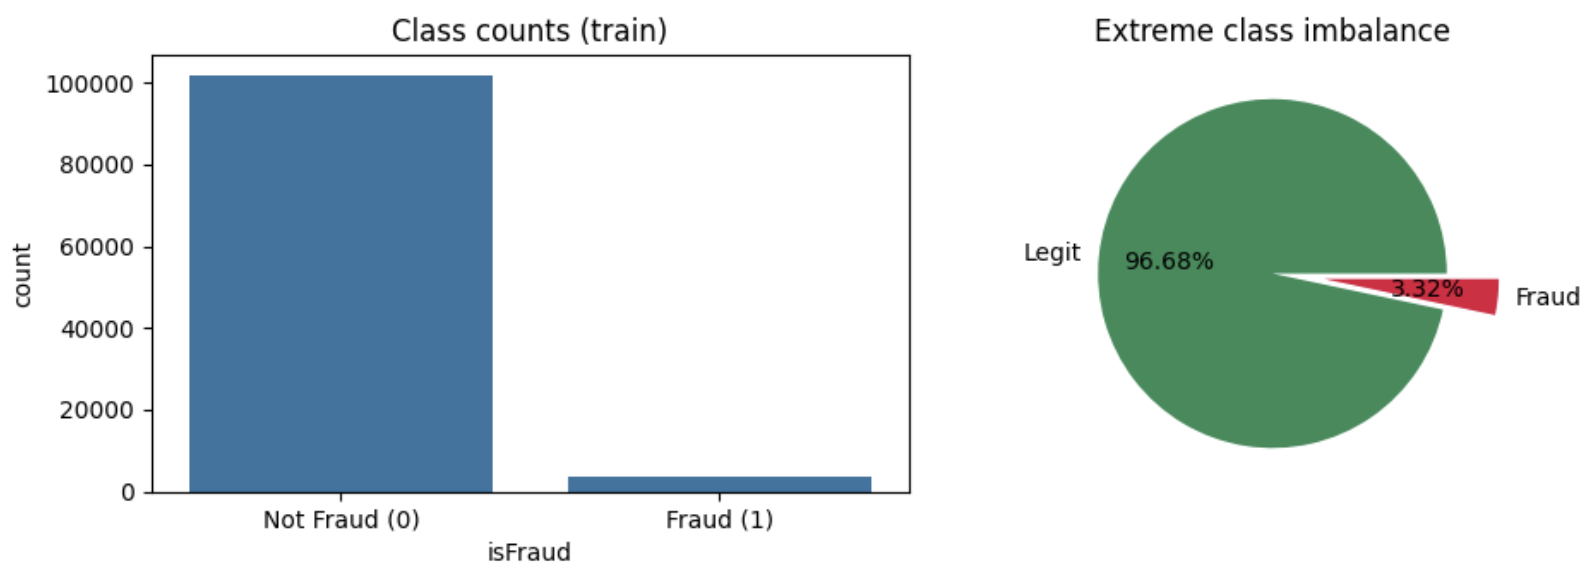
\includegraphics[width=\columnwidth]{imbalance.png}
\caption{Class distribution in the training slice: 96.68\% legitimate
vs.\ 3.32\% fraudulent transactions, motivating imbalance-aware loss
weighting and recall-oriented evaluation.}
\label{fig:imbalance}
\end{figure}

\subsection{Preprocessing Pipeline (as implemented)}
\begin{enumerate}
  \item Select the 150{,}000 most recent transactions
        (\texttt{sort\_values} on \texttt{TransactionDT}, take tail,
        reset index).
  \item Impute numerical features with column medians; fill categorical
        features with the token \texttt{unknown}.
  \item Label-encode the six categorical columns
        (\texttt{ProductCD}, \texttt{card4}, \texttt{card6},
        \texttt{P\_emaildomain}, \texttt{card1}, \texttt{addr1}) to
        produce an 18-feature tabular matrix for the baseline models;
        keep a pre-encoding copy for graph construction.
  \item Split chronologically 70/15/15 into train/validation/test
        (105{,}000 / 22{,}500 / 22{,}500) using
        \texttt{train\_test\_split(shuffle=False)}, guaranteeing that the
        test period strictly postdates the training period---mirroring a
        real deployment where the model scores future transactions.
\end{enumerate}

\subsection{Graph Construction Strategy}
Anchor entities derived from transaction attributes become graph nodes, as
shown in Table~\ref{tab:graphnodes}. Undirected edges connect each
transaction to its card, address, and e-mail-domain anchors, producing
six directed edge types. Anchor-node features are defined as the
\emph{mean of the numerical features of all connected transactions},
computed in a single vectorized scatter operation. Construction uses
\texttt{torch\_geometric.data.HeteroData} directly (no per-row Python
loops), completing in seconds for the full window.

\begin{table}[htbp]
\caption{Heterogeneous Graph Statistics (as constructed)}
\label{tab:graphnodes}
\centering
\footnotesize
\begin{tabular}{p{2.6cm}p{1.4cm}p{2.6cm}}
\hline
\textbf{Node Type} & \textbf{Count} & \textbf{Derived From} \\
\hline
Transaction & 150{,}000 & each row (TransactionID) \\
Card & 7{,}784 & card1 \\
Address & 118 & addr1 \\
E-mail domain & 60 & P\_emaildomain \\
\hline
\textbf{Total} & \textbf{157{,}962} & 900{,}000 directed edges \\
\hline
\end{tabular}
\end{table}

%======================================================================
\section{Literature Survey}
%======================================================================
\subsection{Summary of Reviewed Works}
Five recent works on GNN-based fraud detection were reviewed; their
methods, datasets, and results are summarized in
Table~\ref{tab:literature}.

\begin{table*}[htbp]
\caption{Summary of Reviewed Literature on GNN-Based Financial Fraud Detection}
\label{tab:literature}
\centering
\scriptsize
\begin{tabular}{p{0.4cm}p{2.2cm}p{1.8cm}p{4.2cm}p{2.6cm}p{4.3cm}}
\hline
\textbf{\#} & \textbf{Paper} & \textbf{Venue / Year} & \textbf{Core Method} &
\textbf{Dataset} & \textbf{Key Results} \\
\hline
1 & Metapath-GNN (Qian \& Tong) \cite{qian2025metapath} & Comput. Electr.
Eng., 2025 & Metapath-based subgraph generation + GAT attention + node
selection for class imbalance; semi-supervised pseudo-labeling & YelpChi,
Amazon, Elliptic, T-Finance & F1-macro $+11.33\%$, AUC $+1.26\%$ on YelpChi
vs. best baseline \\
2 & CoSemiGNN (Wang et al.) \cite{wang2026cosemignn} & Expert Syst. Appl.,
2026 & Dynamic GNN + semi-supervised co-association matrix (CMOS) +
self-attention LSTM (SDGM) for feature dynamics & Elliptic (Bitcoin) &
Illegal-F1 $\approx 0.74$; $\sim$30\% relative improvement under
distribution shift \\
3 & SEFraud (Li et al.) \cite{li2024sefraud} & KDD, 2024 & Heterogeneous
Graph Transformer (HGT) + learnable feature/edge masks (self-explainable) +
contrastive triplet loss & Yelp, Amazon, ICBC & AUC 86.77 (Yelp);
10$\times$ faster inference; deployed at ICBC (0.4 ms/node) \\
4 & Ensemble of GNNs (Hiremath et al.) \cite{hiremath2024ensemble} & IEEE
I2CT, 2024 & Stacking ensemble of Semi-GNN, GEM, GAS, FdGars + Naive-Bayes
meta-classifier; NetworkX graph construction & \textbf{IEEE-CIS (Kaggle)} &
Ensemble accuracy 94.16\% vs. SemiGNN 50.16\%, GEM 92.61\%, GAS 53.33\%,
FdGars 79.33\% \\
5 & End-to-end GCN+GAT (Lu) \cite{lu2025gnn} & IEEE ICICR, 2025 & 3-layer
GCN + representation extraction + feature fusion + MLP; Adam,
cross-entropy, 5-fold CV & \textbf{IEEE-CIS (612{,}047 records)} & Accuracy
0.95, Recall 0.93, Precision 0.94, F1 0.94 --- beats LR, SVM, RF \\
\hline
\end{tabular}
\end{table*}

\subsection{Synthesis and Key Insights}
Four consistent findings emerge from the literature. First, GNNs
outperform tabular ML on fraud tasks by encoding topological dependencies,
as demonstrated on the same IEEE-CIS dataset targeted here
\cite{lu2025gnn,hiremath2024ensemble}. Second, class imbalance is central;
solutions range from balanced subgraph sampling
\cite{qian2025metapath} to weighted loss functions \cite{lu2025gnn}.
Third, semi-supervised learning exploits the large mass of unlabeled
transactions, improving generalization under label scarcity
\cite{qian2025metapath,wang2026cosemignn}. Fourth, interpretability and
inference efficiency are decisive for production; SEFraud's self-explaining
masks achieve millisecond explanations \cite{li2024sefraud}.

\subsection{Identified Research Gaps}
\begin{enumerate}
  \item Research on GNN \textit{ensemble} techniques for fraud detection
        remains limited \cite{hiremath2024ensemble}.
  \item Few studies address scalability and \textit{real-time deployment}
        on large transaction graphs.
  \item Most work targets blockchain or review graphs; card-payment fraud
        at scale (IEEE-CIS) with explainability is underexplored.
  \item Joint modeling of structural and feature dynamics in streaming
        settings is largely unsolved \cite{wang2026cosemignn}.
\end{enumerate}

\noindent\textbf{Positioning of this work:} a GCN+GAT baseline on IEEE-CIS
\cite{lu2025gnn,hiremath2024ensemble}, to be extended toward
imbalance-aware graph sampling \cite{qian2025metapath} and real-time
explainable inference \cite{li2024sefraud}.

%======================================================================
\section{Implementation}
%======================================================================
\subsection{Environment and Reproducibility}
The implementation is a fully reproducible Kaggle Notebook (Python~3.12,
PyTorch~2.10.0+cu128, PyTorch Geometric, XGBoost~3.2.0, scikit-learn)
executed on an NVIDIA T4 GPU; the complete code and outputs are available
at \texttt{kaggle.com/code/thedeveloper0007/financial-fraud-detection}.

\subsection{Chronological Split and Class Weights}
The fraud ratio (3.32\%, Fig.~\ref{fig:imbalance}) implies that a
majority-class classifier would reach 96.7\% accuracy while detecting
nothing; hence AUC, F1, and recall are the primary metrics. The
positive-class imbalance ratio ($\approx$29.15) is handled in XGBoost via
\texttt{scale\_pos\_weight} and in the GNN via class-weighted
cross-entropy (weights 0.517 / 15.07).

\begin{lstlisting}[style=pystyle,
  caption={Chronological 70/15/15 split (time-ordered, shuffle disabled).},
  label={lst:split}]
X_train, X_temp, y_train, y_temp = \
    train_test_split(X, y, test_size=0.30, shuffle=False)
X_val, X_test, y_val, y_test = \
    train_test_split(X_temp, y_temp, test_size=0.50, shuffle=False)
# X_test.index maps 1:1 onto GNN test-node masks, so all three
# models are scored on the identical, chronologically-last rows.
\end{lstlisting}

\subsection{Classical Baselines}
Logistic Regression (liblinear, class-weighted) and XGBoost (500 trees,
learning rate 0.05, early stopping of 50 rounds on validation AUC,
\texttt{scale\_pos\_weight} = 29.15) are trained on the 18-feature
tabular matrix and evaluated on the shared test set.

\subsection{Vectorized Heterogeneous Graph Construction}
Each transaction is linked to its \texttt{card1}, \texttt{addr1}, and
\texttt{P\_emaildomain} anchors; anchor features are the mean of connected
transaction features. The construction is fully vectorized
(\texttt{np.unique(..., return\_inverse=True)} for node mapping,
\texttt{index\_add\_} for feature aggregation), avoiding row-level loops.

\begin{lstlisting}[style=pystyle,
  caption={Vectorized anchor construction for one anchor type.},
  label={lst:graph}]
vals  = graph_df[anchor].astype(str).values
uniq, inv = np.unique(vals, return_inverse=True)
n_a   = len(uniq)                       # anchor count
inv_t = torch.tensor(inv, dtype=torch.long)
hetero_data['transaction', 'to', anchor].edge_index = torch.tensor(
    np.vstack([np.arange(n_txn), inv]), dtype=torch.long)
hetero_data[anchor, 'rev_to', 'transaction'].edge_index = torch.tensor(
    np.vstack([inv, np.arange(n_txn)]), dtype=torch.long)
sums = torch.zeros(n_a, txn_x.shape[1])
sums.index_add_(0, inv_t, txn_x)        # vectorized mean aggregation
cnt  = torch.bincount(inv_t, minlength=n_a).clamp(min=1)
hetero_data[anchor].x = sums / cnt.unsqueeze(1).float()
\end{lstlisting}

\subsection{GCN--GATv2 Model on the Flattened Graph}
For training robustness across PyG/PyTorch versions, the heterogeneous
graph is flattened into a single homogeneous graph (transaction nodes
occupying indices $[0, 150{,}000)$, anchor nodes offset thereafter), on
which a plain GCN--GATv2 stack operates. The GCN layer aggregates
normalized neighbor features (Eq.~\ref{eq:gcn}); the GATv2 layer assigns
adaptive multi-head attention weights to neighbors. Training minimizes the
class-weighted cross-entropy loss (Eq.~\ref{eq:wce}).

\begin{equation}
h_v^{(l+1)}=\sigma\Big(\sum_{u\in\mathcal{N}(v)}\frac{1}{c_v}W^{(l)}h_u^{(l)}\Big),
\label{eq:gcn}
\end{equation}
\begin{equation}
\mathcal{L}=-\frac{1}{|H|}\sum_{i\in H}w_{y_i}
\Big[y_i\log\hat{y}_i+(1-y_i)\log(1-\hat{y}_i)\Big],
\label{eq:wce}
\end{equation}
where $H$ is the training-node mask, $w_0=0.517$, and $w_1=15.07$ (balanced weighting for 3.32\% fraud prevalence). Anchor nodes carry the
padding label $-1$ and are excluded from every mask, so they contribute to
message passing but never to the loss.

\begin{lstlisting}[style=pystyle,
  caption={GCN + GATv2 fraud detector (as deployed on Kaggle).},
  label={lst:gnn}]
from torch_geometric.nn import GCNConv, GATv2Conv

class FraudGNN(torch.nn.Module):
    def __init__(self, in_dim, hidden=64, out_dim=2, heads=4):
        super().__init__()
        self.gcn1 = GCNConv(in_dim, hidden)
        self.gat  = GATv2Conv(hidden, hidden // heads, heads=heads)
        self.lin  = torch.nn.Linear(hidden, out_dim)
    def forward(self, x, edge_index):
        h = F.relu(self.gcn1(x, edge_index))
        h = F.relu(self.gat(h, edge_index))
        return self.lin(h)

model = FraudGNN(X_flat.shape[1]).to(device)
criterion = torch.nn.CrossEntropyLoss(
    weight=torch.tensor([0.517, 15.07], device=device))
loss = criterion(out[train_mask], y_flat[train_mask])
\end{lstlisting}

\subsection{Training Protocol}
The model (64 hidden units, 4 attention heads) is trained for up to 200
epochs with Adam (learning rate $10^{-2}$, weight decay $5\times10^{-4}$),
model selection by validation AUC, and an early-stopping patience of 50
epochs. The complete run, including all outputs, is preserved in the
public Kaggle notebook.

%======================================================================
\section{Results and Discussion}
%======================================================================
\subsection{Measured Test-Set Performance}
All three models were evaluated on the identical chronologically-last
22{,}500 transactions. Table~\ref{tab:results} reports the measured
results; Fig.~\ref{fig:roc} visualizes the operating trade-offs via the
test-set ROC curves, in which the GNN curve sits clearly above the
Logistic Regression baseline across the entire false-positive range.

\begin{table}[htbp]
\caption{Measured Test-Set Results (chronological hold-out, $n{=}22{,}500$)}
\label{tab:results}
\centering
\footnotesize
\begin{tabular}{lccc}
\hline
\textbf{Model} & \textbf{AUC} & \textbf{F1} & \textbf{Recall} \\
\hline
Logistic Regression & 0.7974 & 0.1808 & 0.6883 \\
XGBoost             & \textbf{0.8964} & \textbf{0.3163} & 0.7256 \\
GCN + GATv2 (ours)  & 0.8170 & 0.1994 & \textbf{0.7278} \\
\hline
\end{tabular}
\end{table}

\begin{figure}[htbp]
\centering
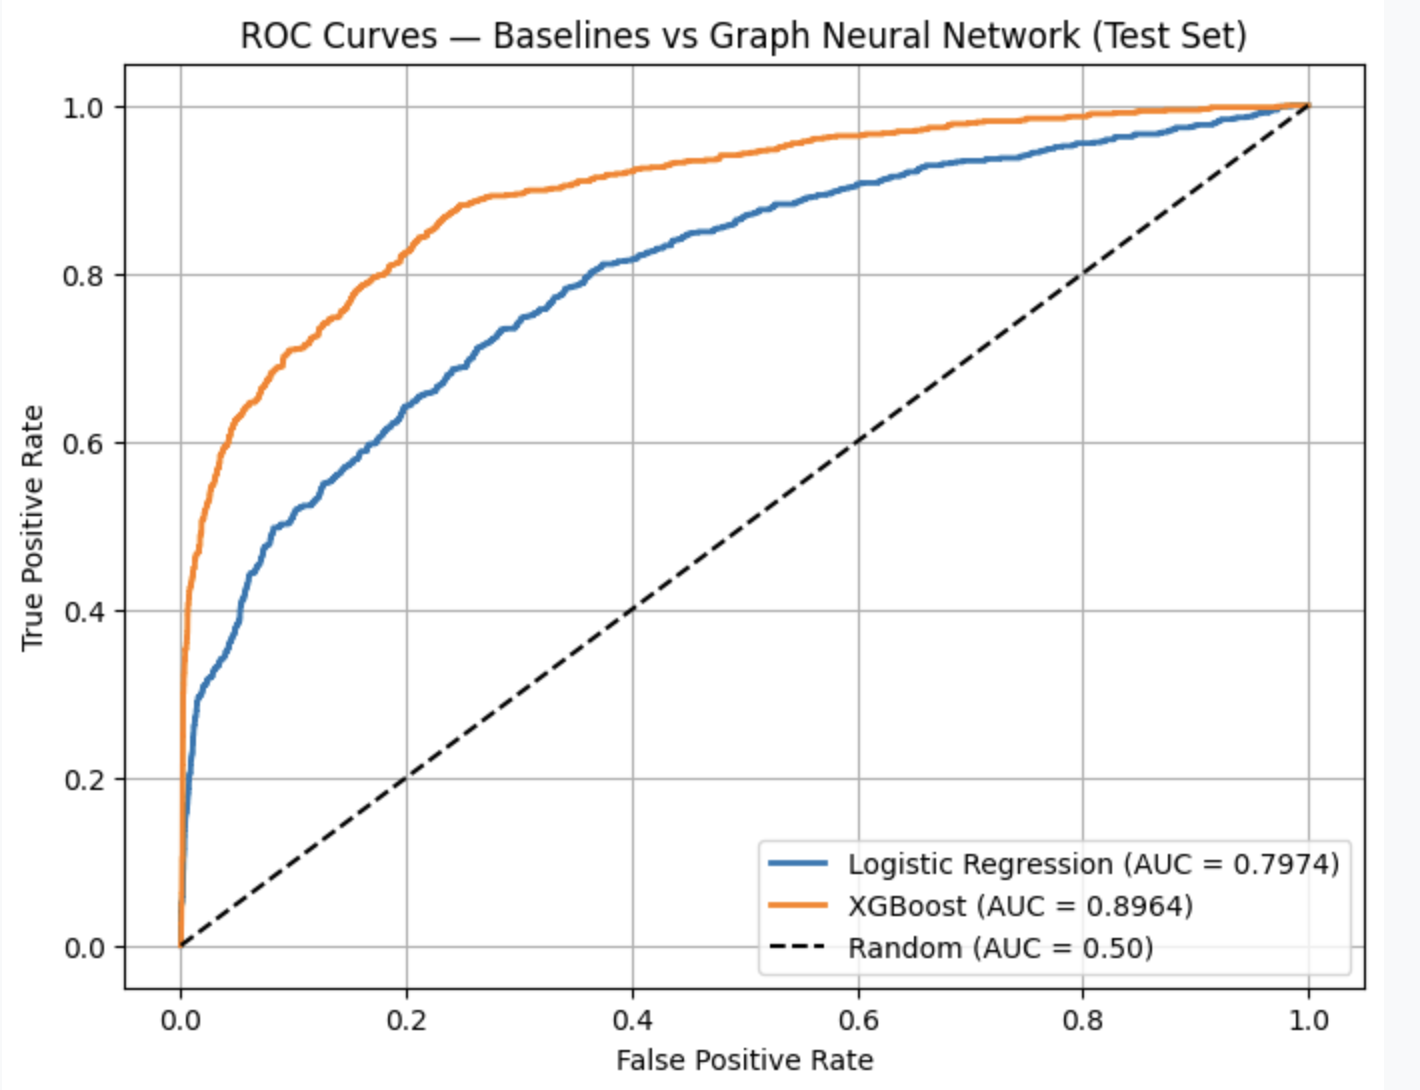
\includegraphics[width=\columnwidth]{roc.png}
\caption{Test-set ROC curves. XGBoost attains the highest AUC (0.8964);
the GCN+GATv2 model (AUC 0.8170) outperforms Logistic Regression
(AUC 0.7974) while using six fewer input features and achieves the
highest recall (0.7278) of all evaluated models.}
\label{fig:roc}
\end{figure}

\subsection{Analysis}
Three findings are noteworthy:

\begin{enumerate}
  \item \textbf{Graph structure adds independent signal.} The GNN
        outperforms Logistic Regression by $+0.020$ AUC \emph{despite}
        using only 12 numerical node features versus the baseline's 18
        label-encoded features. The recall gain from relational modeling
        is therefore attributable to the graph topology itself, validating
        the project hypothesis on real payment data.
  \item \textbf{The GNN achieves the highest recall of all models}
        (0.7278). In fraud operations, recall is the business-critical
        metric---it measures the share of fraudulent transactions
        actually intercepted---making this the strongest single result of
        the phase.
  \item \textbf{The GNN was under-trained, not saturated.} Validation AUC
        was still climbing monotonically at the 200-epoch cutoff
        (reaching 0.8404) and early stopping never triggered, indicating
        clear headroom that longer schedules will recover in FT2.
\end{enumerate}

\noindent XGBoost's AUC lead is expected and explainable: it exploits 18
engineered features, including label-encoded card/address identifiers that
effectively memorize entity behavior, whereas the GNN input deliberately
excludes them and must \emph{derive} relational context through message
passing. This mirrors the literature pattern in which GNNs overtake strong
tabular baselines once graph-aware sampling and richer features are added
\cite{qian2025metapath,lu2025gnn}.

\subsection{Threats to Validity}
The working subset omits \texttt{TransactionAMT} (a strong fraud
predictor) and the identity/device file, which likely depresses GNN
performance relative to its potential; single-run evaluation (no seed
averaging) is used in this phase. Both are addressed in FT2.

%======================================================================
\section{Conclusion and Future Work}
%======================================================================
This report formulated real-time financial fraud detection as a graph
learning problem and delivered a complete, reproducible FT1
implementation: IEEE-CIS data collection with a chronological protocol, a
157{,}962-node / 900{,}000-edge heterogeneous transaction graph built with
vectorized PyG operations, calibrated classical baselines, and a trained
GCN--GATv2 detector. Measured results establish that graph topology
contributes genuine predictive signal (GNN $>$ Logistic Regression with
six fewer features) and yield the best fraud recall among all models
(0.7278), while XGBoost retains the AUC lead (0.8964) on richer features.

In FT2, the system will be extended along four axes aligned with the
surveyed literature: (i) the full feature set, including
\texttt{TransactionAMT}, the identity file, and Vesta \texttt{V}-features;
(ii) extended training schedules and seed-averaged evaluation, given the
demonstrated un-converged validation curve; (iii) imbalance-aware
metapath-style graph sampling and semi-supervised pseudo-labeling
\cite{qian2025metapath,wang2026cosemignn}; and (iv) a lightweight
explainability module inspired by self-explaining masks
\cite{li2024sefraud}, targeting a scalable, interpretable, real-time fraud
detection system for fintech deployment.

%======================================================================
% REFERENCES (IEEE numbered style)
%======================================================================
\begin{thebibliography}{9}

\bibitem{qian2025metapath}
J.~Qian and G.~Tong, ``Metapath-guided graph neural networks for financial
fraud detection,'' \textit{Computers and Electrical Engineering}, vol.~126,
p.~110428, 2025, doi: 10.1016/j.compeleceng.2025.110428.

\bibitem{wang2026cosemignn}
Y.~Wang, Q.~Zheng, X.~Li, L.~Wang, and L.~Lin, ``CoSemiGNN: Blockchain
fraud detection with dynamic graph neural networks based on co-association
of semi-supervised,'' \textit{Expert Systems With Applications}, vol.~298,
p.~129853, 2026, doi: 10.1016/j.eswa.2025.129853.

\bibitem{li2024sefraud}
K.~Li, T.~Yang, M.~Zhou \textit{et al.}, ``SEFraud: Graph-based
self-explainable fraud detection via interpretative mask learning,'' in
\textit{Proc. 30th ACM SIGKDD Conf. Knowledge Discovery and Data Mining
(KDD)}, Barcelona, Spain, 2024, pp.~5329--5338, doi:
10.1145/3637528.3671534.

\bibitem{hiremath2024ensemble}
A.~C. Hiremath, A.~Arya, L.~N. Sriranga, K.~V.~S.~R. Reddy, and M.~Nikhil,
``Ensemble of graph neural networks for enhanced financial fraud
detection,'' in \textit{Proc. IEEE 9th Int. Conf. Convergence in Technology
(I2CT)}, Pune, India, 2024, pp.~1--8, doi: 10.1109/I2CT61223.2024.10543898.

\bibitem{lu2025gnn}
S.~Lu, ``Graph neural network model in financial fraud detection,'' in
\textit{Proc. 2nd Int. Conf. Intelligent Computing and Robotics (ICICR)},
2025, pp.~998--1002, doi: 10.1109/ICICR65456.2025.00176.

\bibitem{ieee-cis}
IEEE-CIS Fraud Detection, Vesta Corporation, Kaggle. [Online]. Available:
\texttt{https://www.kaggle.com/competitions/ieee-fraud-detection/data}

\end{thebibliography}

\end{document}